\documentclass[spanish]{scrartcl}
\usepackage[utf8]{inputenc}
\usepackage{babel}
\usepackage[paper=a4paper, top=2cm, left=2cm, right=2cm]{geometry}
\usepackage{tikz}
\usepackage{CIACcustom}
\usepackage{fourier}
\usepackage{amsmath, amsthm}
\usepackage{listings}
\usepackage{multicol}
\usepackage{fancyhdr}
\usepackage[urlcolor=blue, colorlinks]{hyperref}
\usepackage{booktabs,tabularx}
\usepackage{float}
\usepackage{verbatim}

\newcolumntype{L}[1]{>{\hsize=#1\hsize\raggedright\arraybackslash}X}%
\newcolumntype{R}[1]{>{\hsize=#1\hsize\raggedleft\arraybackslash}X}%
\newcolumntype{C}[2]{>{\hsize=#1\hsize\columncolor{#2}\centering\arraybackslash}X}%

\pagestyle{fancy}
\fancyhf{}
\rhead{\pgfimage[width=2.5cm]{imagenes/logo-ciac.png}}
\chead{
  Apoyos Intensivos Online Guía N° 1\\
  IWI-131 Semestre II-2019 Fase I \\
  CIAC Casa Central
}
\lhead{\pgfimage[width=2.5cm]{imagenes/logo-usm.jpg}}
\rfoot{\LaTeXe / CIAC 2019}
\lfoot{Página \thepage}
\renewcommand{\headrulewidth}{0.5pt}
\renewcommand{\footrulewidth}{0.5pt}

\renewcommand{\ttdefault}{pcr}

%%% listings settings:
\definecolor{bggray}{rgb}{0.95,0.95,0.95}
\lstdefinestyle{consola}{
  backgroundcolor=\color{bggray},
  basicstyle=\small\ttfamily,
  frame=single,
  moredelim=[is][\bfseries]{[*}{*]},
  xrightmargin=5pt
}

\lstdefinestyle{mypy}{
  language=python,
  backgroundcolor=\color{bggray},
  basicstyle=\ttfamily\small\color{orange!70!black},
  frame=L,
  keywordstyle=\bfseries\color{green!40!black},
  commentstyle=\itshape\color{purple!40!black},
  identifierstyle=\color{blue},
  stringstyle=\color{red},
  numbers=left,
  showstringspaces=false,
  xrightmargin=5pt,
  xleftmargin=10pt
}

\setlength{\headheight}{47pt}

\newtheorem{CIACdef}{Definición}

\begin{document}
% \vspace*{-.3cm}
\vspace*{-0.4cm}
\section*{Pregunta 1}

\begin{enumerate}
    \item A continuación se presenta el ruteo correspondiente:
\begin{center}
    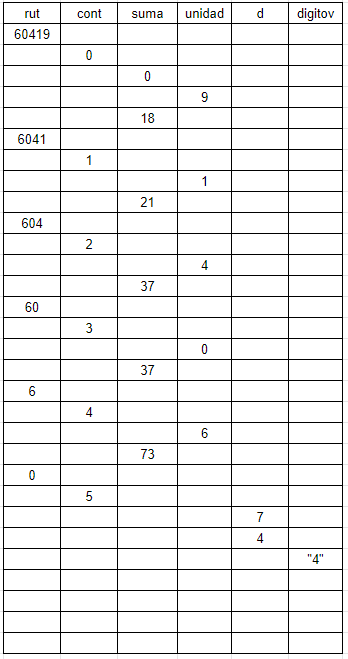
\includegraphics[scale=0.84]{Imagenes/ruteo_pauta}
\end{center}

    El programa imprime \texttt{4}.

    \item El código calculaba el dígito verificador del RUT. También era aceptable responder que, en base a cierto numero, este programa entrega un caracter que podría ser un dígito o una k.

\end{enumerate}

\newpage
\section*{Pregunta 2}

A continuación se presenta una forma posible de resolver el problema propuesto:
\lstinputlisting[
    style  = mypy,
    caption= \texttt{biblioteca.py}]{Code/p2.py}

\newpage
\section*{Pregunta 3}

A continuación se presenta una forma posible de resolver el problema propuesto:
\lstinputlisting[
    style  = mypy,
    caption= \texttt{tepyton.py}]{Code/p3.py}
\newpage
\section{Matrices}

Las funciones solicitadas y el máximo correspondiente (70600674) se calculan con el siguiente código

\lstinputlisting[style=mypy,caption=\texttt{matrices.py}]{Code/matrices.py}


\end{document}
